\documentclass{tpk4170report}

\title{Title of Report}
\author{Author(s)}

\usepackage{blindtext}

\addbibresource{references.bib} 

\begin{document}

\maketitle

\frontmatter

\chapter*{Preface}

\tableofcontents
\listoffigures
\listoftables

\mainmatter








\chapter{Introduction}
\label{chap:Introduction}

\blindmathtrue
\blindtext

This is a citation~\cite{McCarthy2011}. \blindtext

See Table~\ref{table:floating-table} for a floating table and
\eqref{eq:equation-example} for an equation.
\begin{align}
  \label{eq:equation-example}
  y = ax + b 
    = cz + d 
\end{align}

\begin{table}
  \centering
  \begin{tabular}{l|lll}
    a& b& c &d \\
    \hline
    a& b& c &d \\
    a& b& c &d \\
    a& b& c &d
  \end{tabular}
  \caption{This is a floating table}
  \label{table:floating-table}
\end{table}




\chapter{Forward Kinematics}
\section{Task 1}

Denavit-Hartenberg (DH) is a convention broadly used in robotics. It was introduced in order to standardize the attachmemt of cordinate frames to robots. A robot can be seen as a kinematic chain of rigid bodies. These rigid bodies are called links and are connected with joints. A robot arm is represenetd by a kinematic chain which is a concatenation of several links and joints. If one object is manipulated by one robot the system is called open kinematic chain. If several robots manipulate one object simultanously the system is called closed kinematic chain. In this task we will focus on open chain robots. Forward kinematics is a way of of calculating the end effector pose based on the joint parameters. The relation from the end effector to the base is done by attaching one frame to the end effector and one to the base of the robot. The relation between those two frames is then determined by the homogenious transformation matrix \(T_{E}^{B}\). To make things easier a frame can be attached to each link and then the relation between each consecutive frame can be calculated by \(T_{i+1}^{i}\). Concatenating all these homogenious Transformations and building their dot product determines the homogenious Transformation from the robot base to end effector: 
\begin{equation}
  T_{E}^{B} = T_{0}^{1}*T_{1}^{2}* ... *T_{i-1}^{i}
  \label{eqn:recursive_expression_homogenious_transformation}
\end{equation}
Denavit-Hartenberg (DH) is a convention which standardizes the attachmemt of cordinate frames to a robot. It is a convention broadly used in the community which makes the application of the recursive formula in \ref{eqn:recursive_expression_homogenious_transformation} more intuitive. The DH convention provides rules how to attach the frames to the link. In general the result should be the same if the frames are attached differently to the links as long as every link is considered. In the DH convention four different parameters afe used in order to attach frames to the robot links. The frame of the link i+1 is determined based on the frame of the link i. The placement of a frame is visualized in figure \ref{fig:Denavit_Hartenberg_Konvention_Rules}. The followinfg consecutive rules are applied:

\begin{itemize}
  \item[1] \(z_{i}\) alligns with the rotational axis of joint i+1
  \item[2] \(O_{i}\) is placed at the intersetion of \(z_{i}\) and the common normal of \(z_{i-1}\) and \(z_{i}\) 
  \item[3] \(O_{i'}\) is placed at the intersetion of \(z_{i-1}\) and the common normal of \(z_{i-1}\) and \(z_{i}\)
  \item[4] \(x_{i}\) alligns with the common normal of \(z_{i-1}\) and \(z_{i}\) pointing away from \(O_{i}\)
  \item[5] \(y_{i}\) is chosen according to the right hand rule for coordinate frames
  \end{itemize}
\begin{figure}
  \centering
  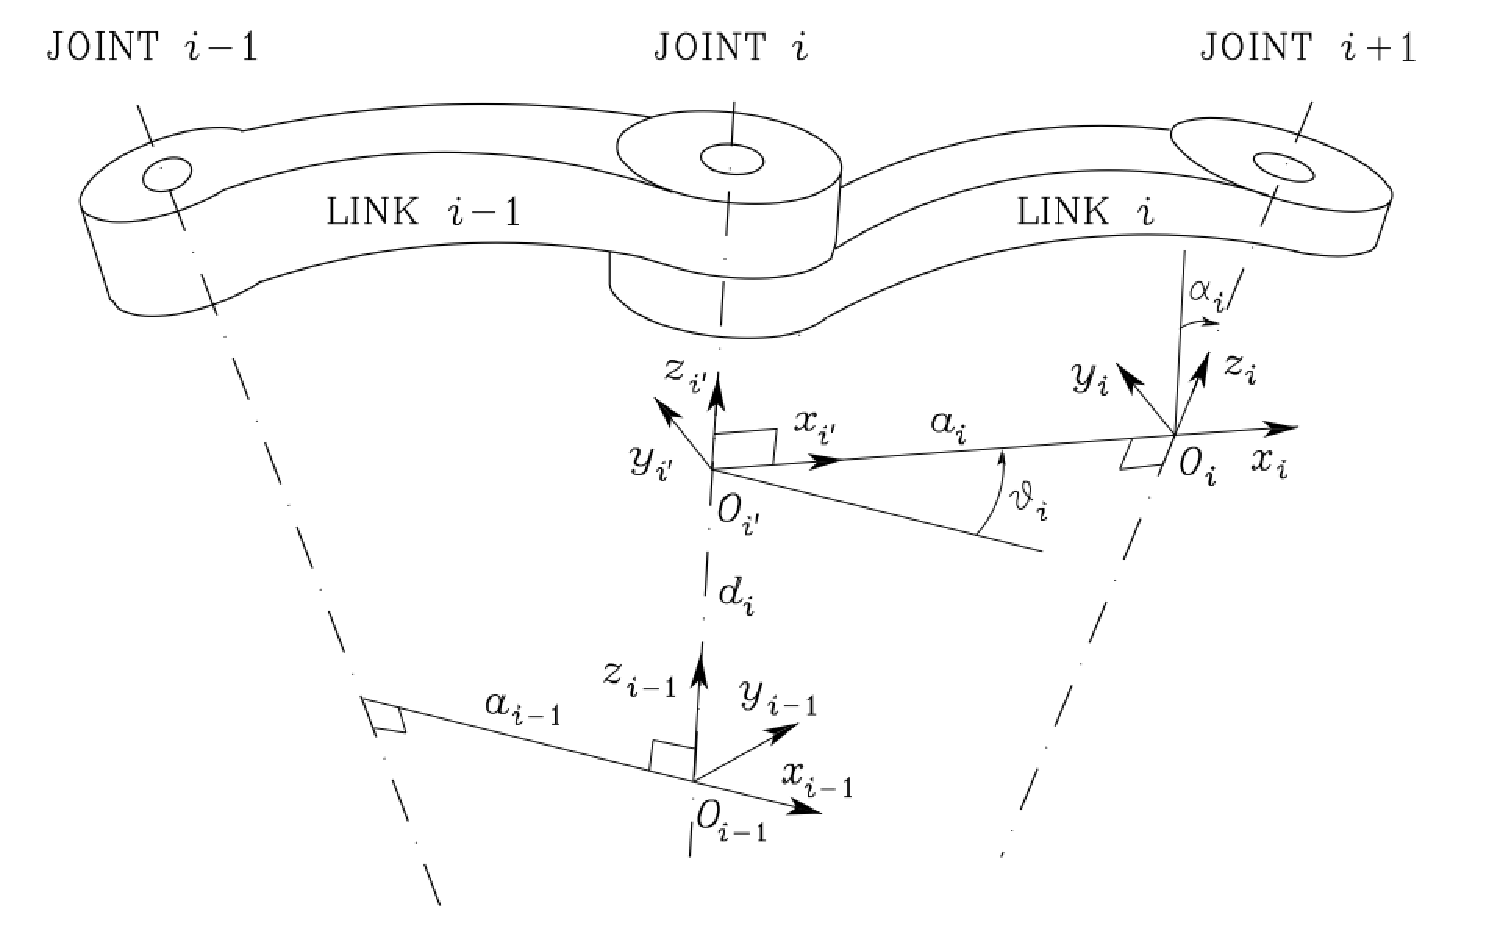
\includegraphics[width=0.8\textwidth]{assets/Denavit_Hartenberg_Convention_Rules.pdf} 
  \caption{Denavit Hartenberg convention rules \cite{Siciliano2009}}
  \label{fig:Denavit_Hartenberg_Konvention_Rules}
\end{figure}

The DH convention does not define enough rules to make sure that there is just one uniquie solution. 

\begin{itemize}
  \item[1] There is no frame i-1 for frame 0 we can not define \(O_{0}\) and \(x_{0}\):  \(O_{0}\) and \(x_{0}\) can be defined arbitrarily.
  \item[2] There is no joint i+1 when defining frame n we can not define \(z_{n}\): \(z_{n}\) is defined parallel to \(z_{n-1}\) . 
\end{itemize}  Usually there are some ways of defining those two parameters which make applying the convention easier.

There are some special cases which also do not allow a unique definition of frames:
\begin{itemize}
  \item[1] \(z_{i+1}\) and \(z_{i}\) are parallel: \(O_{i}\) and \(x_{i}\) can be selected arbitrarily.
  \item[2] \(z_{i+1}\) and \(z_{i}\) intersect: \(O_{i}\) and \(x_{i}\) can be selected arbitrarily.
  \item[3] joint i is prismatic: \(x_{i-1}\) can be selected arbitrarily.
\end{itemize}

The DH convention makes finding the homogenious transformations especially convenient. After establishing the frames at each joint the four DH parameters can be identified. 

\begin{itemize}
  \item[\(a_{i}\)]: distance between \(O_{i}\) and \(O_{i'}\) 
  \item[\(d_{i}\)]: distance between \(O_{i'}\) and \(O_{i-1}\) along \(z_{i-1}\)
  \item[\(\alpha_{i}\)]: angle between \(z_{i-1}\) and \(z_{i}\) about \(x_{i}\)
  \item[\(\vartheta{i}\)]:  angle between \(x_{i-1}\) and \(x_{i}\) about \(z_{i-1}\)
\end{itemize}

The paramters \(a_{i}\) and \(\alpha_{i}\) are constant and just depend on the geometry of the link i. Non constant is the parameter \(d_{i}\) if joint i is prismatic and the parameter \(\vartheta{i}\) if joint i is rotational.

Having the four parameters \(a_{i}\), \(d_{i}\), \(\alpha_{i}\), \(\vartheta_{i}\)one can write down the homogenious transformations T immediatelly: 

\begin{equation}
  T_{i}^{i-1}= 
  \begin{bmatrix}
    c_{\vartheta_{i}} & -s_{\vartheta_{i}}c_{\alpha_{i}} &  s_{\vartheta_{i}}s_{\alpha{i}} & a_{i}c_{\vartheta_{i}} \\
    s_{\vartheta_{i}} & c_{\vartheta_{i}}c_{\alpha{i}} & -c_{\vartheta_{i}}s_{\alpha{i}} & a_{i}s_{\vartheta_{i}} \\
    0 & s_{\alpha{i}} & c_{\alpha{i}} & d_{i} \\
    0 & 0 & 0 & 1
  \end{bmatrix}
  \label{eqn:Transformation_Denavit_Hartenberg}
\end{equation}
\cite{Siciliano2009}

\section{Task 2}
The modified DH convention presented in \cite{Lynch2017} differs to the original DH presented in \cite{Siciliano2009}. In figure \ref{fig:Denavit_Hartenberg_Konvention_Rules_modified} The frames are attached to the links differntly (see table \ref{table:frame_attachment_DH}). Getting the DH parameters from the attached frames therefore also differs (see table \ref{table:DH_parameters}). Like mentioned before the attachment of the frames does not change the forward dynamics. Anyway, sticking with one convention makes calculatations more intuitive and easier to understand for others.

\begin{figure}
  \centering
  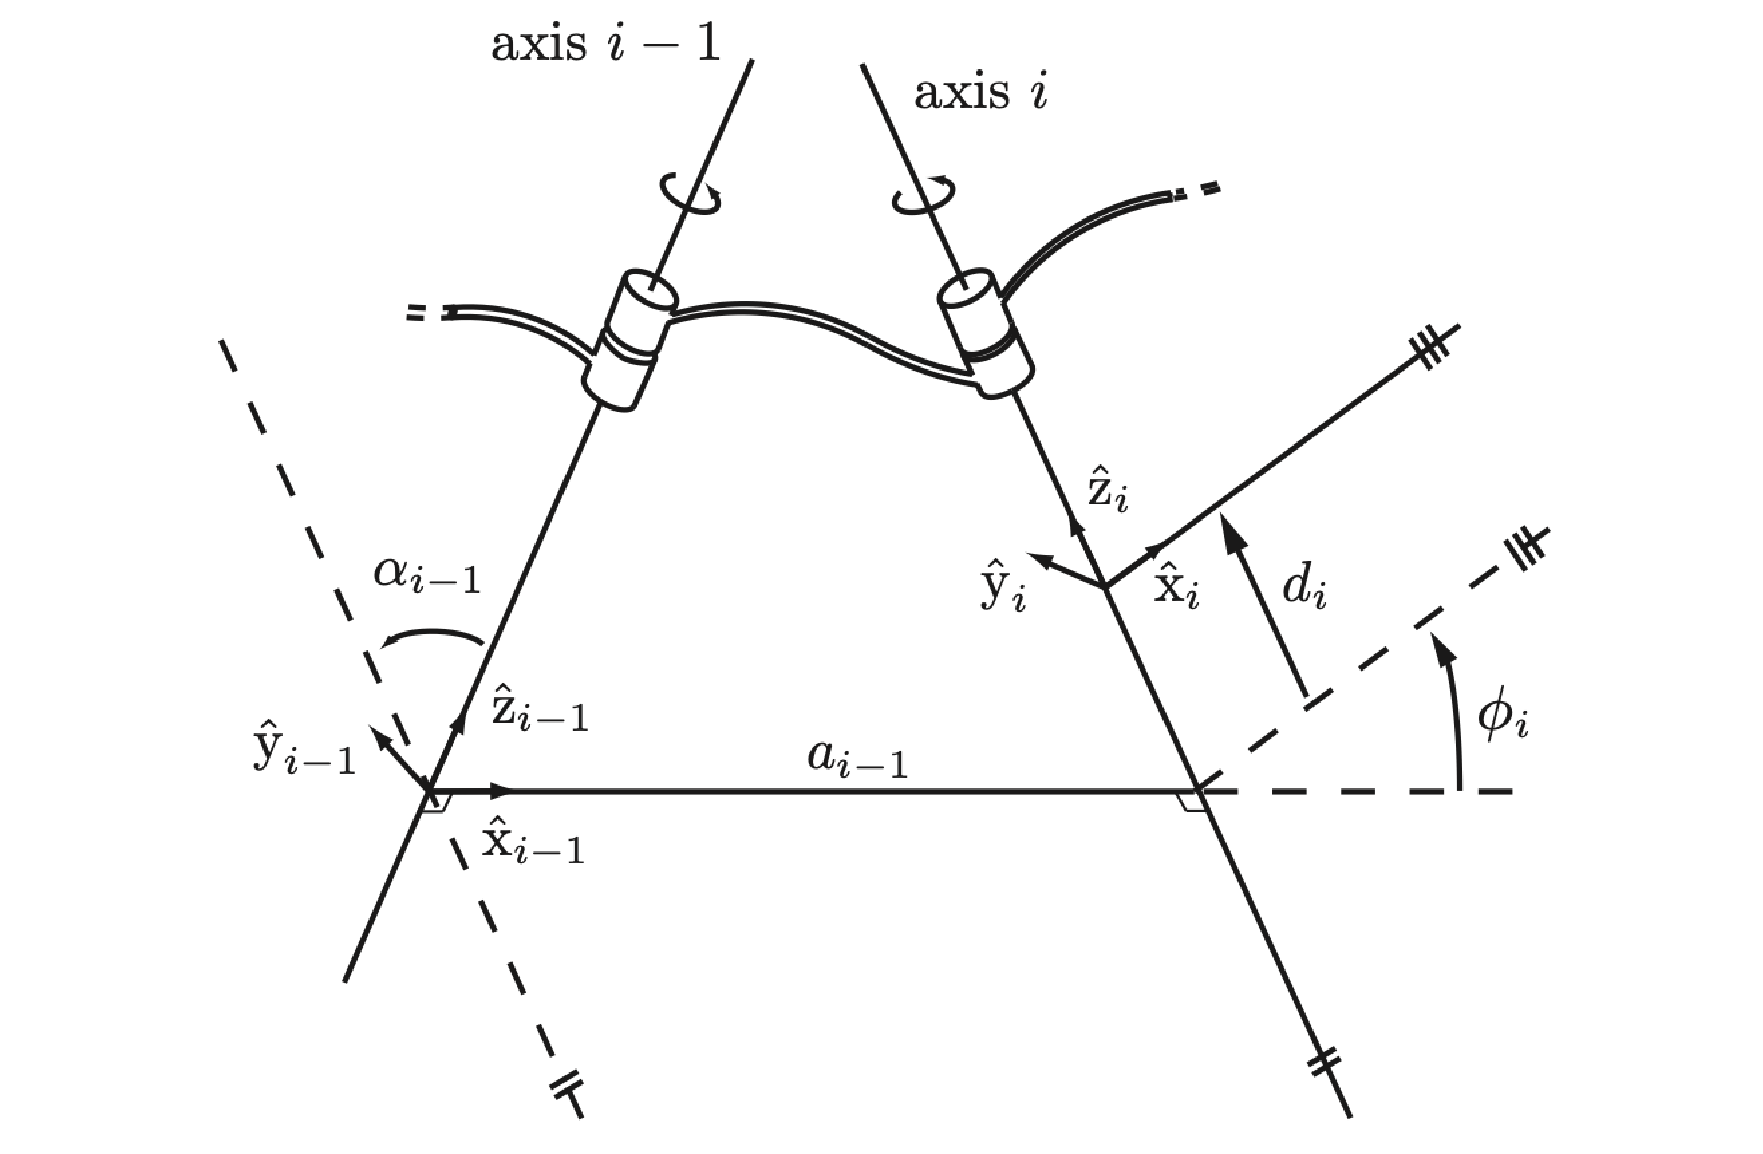
\includegraphics[width=0.8\textwidth]{assets/Denavit_Hartenberg_Convention_Rules_Modified.pdf} 
  \caption{Modified Denavit Hartenberg convention rules \cite{Lynch2017}}
  \label{fig:Denavit_Hartenberg_Konvention_Rules_modified}
\end{figure}

In the following passage the differences in the frame attachement are presented.

\begin{table}
  \centering
  \begin{tabular}{l|lll}
    \vtop{\hbox{\strut frame }\hbox{\strut parameters }} & original DH & modified DH \\
    \hline
    \(z_{i}\) & \vtop{\hbox{\strut alligns with the rotational axis}\hbox{\strut of joint i+1}} & \vtop{\hbox{\strut alligns with the rotational axis}\hbox{\strut of joint i}} \\
    \(O_{i}\) & \vtop{\hbox{\strut is placed at the intersetion of \(z_{i}\) }\hbox{\strut and the common normal of \(z_{i-1}\) and \(z_{i}\)}} &  \vtop{\hbox{\strut is placed at the intersetion of \(z_{i}\) }\hbox{\strut and the common normal of \(z_{i}\) and \(z_{i+1}\)}}\\
    \(x_{i}\) & \vtop{\hbox{\strut alligns with the common normal of }\hbox{\strut \(z_{i-1}\) and \(z_{i}\) pointing away from \(O_{i}\) }} & \vtop{\hbox{\strut alligns with the common normal of }\hbox{\strut \(z_{i+1}\) and \(z_{i}\) and pointing away from \(O_{i}\) }}\\
  \end{tabular}
  \caption{frame attachment original versus modified DH}
  \label{table:frame_attachment_DH}
\end{table}


\begin{table}
  \centering
  \begin{tabular}{l|lll}
    \vtop{\hbox{\strut DH }\hbox{\strut paramters }} & original DH & modified DH \\
    \hline
    \(a_{i}\)& length of common normal of \(z_{i-1}\) and \(z_{i}\) & length of common normal of \(z_{i}\) and \(z_{i+1}\) \\
    \(d_{i}\) &  \vtop{\hbox{\strut distance between \(O_{i-1}\) and intersection of }\hbox{\strut common normal of \(z_{i-1}\) and \(z_{i}\) with \(z_{i-1}\)}} &  \vtop{\hbox{\strut distance between \(O_{i}\) and intersection of }\hbox{\strut common normal of \(z_{i-1}\) and \(z_{i}\)  with \(z_{i}\)}}\\
    \(\alpha_{i}\) & angle between \(z_{i-1}\) and \(z_{i}\) about \(x_{i}\) &  angle between \(z_{i-1}\) and  \(z_{i}\) about \(x_{i-1}\) \\
    \(\vartheta{i}\) & angle between \(x_{i-1}\) and \(x_{i}\) about \(z_{i-1}\)  &  angle between \(x_{i-1}\) and \(x_{i}\) about \(z_{i}\) \\
  \end{tabular}
  \caption{DH parameter original versus modified DH}
  \label{table:DH_parameters}
\end{table}

In the special case where two consecutive \(z_{i}\) and \(z_{i-1}\) intersect \cite{Lynch2017} recommends to pick a \(x_{i-1}\) which is perpendicular to the plane spanned by \(z_{i}\) and\(z_{i-1}\). \cite{Siciliano2009} just says that an arbitrary \(x_{i}\) should be picked.


\section{Task 3}

\subsection{Twist}
Rigid body motions can be expressed by consecutively applying a rotation and translation on a body. So called twists which use rotations around a srew axis and translation along the screw axis can also be used to represent rigid body motions. The screw axis \(S\) can be represented by three parameters \(q, \hat{s}, h\), where \(q\) is any point on the screw axis, \(\hat{s}\) is the unit vector representing the screw axis and \(h\) is the screw pitch, which deifines the ratio of linear and angular velocity. Figure \ref{fig:Twist} shows:
\begin{itemize}
  \item[-] angular velocity \(\dot{\theta}\) which rotates the coordinate frame around the screw axis
  \item[-] the angular speed due to the angualar velocity: \(\dot{\theta}\): -\( \hat{s} \dot{\theta} \times q \)
  \item[-] the linear speed due to the screw pitch \(h\): \( h \hat{s} \dot{\theta} \)
\end{itemize}

The twist can than be written as:
\[
V
=
\begin{bmatrix}
  w \\
  v
\end{bmatrix}
=
\begin{bmatrix}
  \hat{s} \dot{\theta}\\
  - \hat{s} \dot{\theta} \times q + h \hat{s} \dot{\theta}
\end{bmatrix}
\]
Instead of representing the screw axis with \(q, \hat{s}, h\) we can also represent it as a normalized version of any twist. Still the previous example gives a good intuition for twists and screw axis. This will help to understand the PoE formula later in this section. 



\begin{figure}
  \centering
  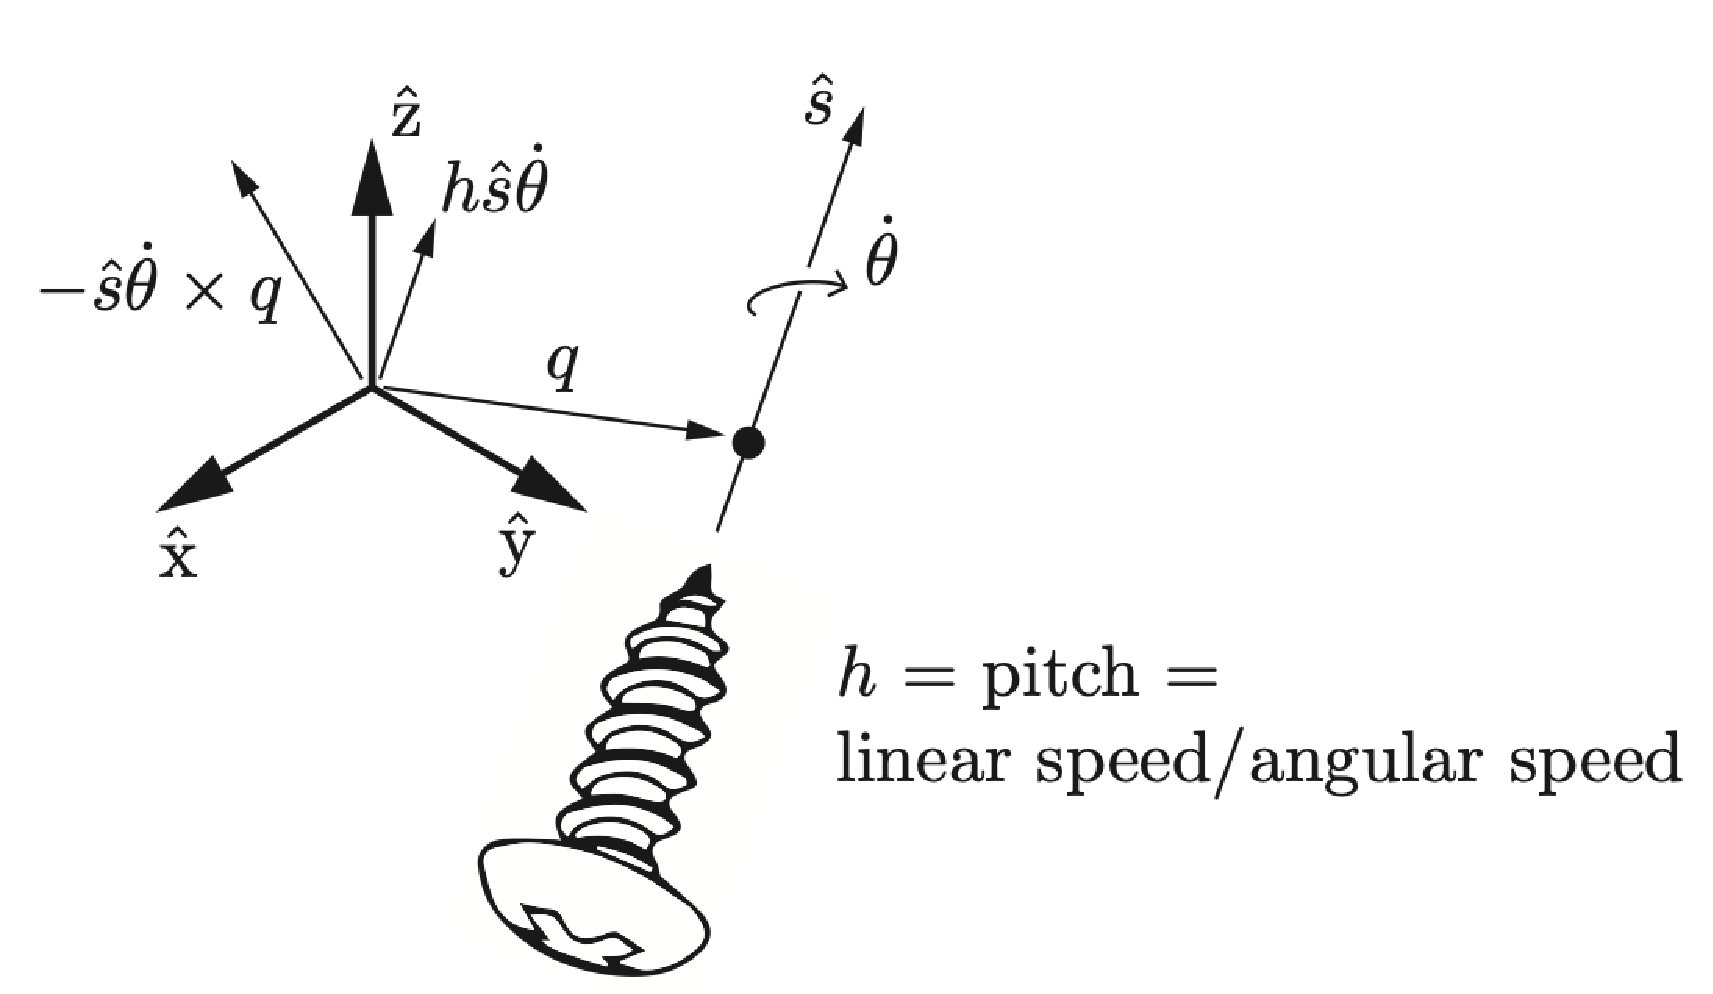
\includegraphics[width=0.7\textwidth]{assets/Twist.pdf} 
  \caption{Screw axis Visualization \cite{Lynch2017}}
  \label{fig:Twist}
\end{figure}

\subsection{Exponential Coordinates of Twists}
Applying the matrix exponential to \( w \dot{\theta}\) the corresponding rotation matrix is generated. Equivalently this works for Twists. Applying the matrix exponential to \( S \theta \in \mathbb{R}^{6} \) we receive the homogenious Transformation \( T\)

\begin{itemize}
  \item[exp]: \([S] \theta \in se(3) \Rightarrow T \in SE(3)\)
  \item[log]: \(T \in SE(3) \Rightarrow [S] \theta \in se(3)\)
\end{itemize}

In the next section the PoE formula is presented for solving the forward kinematics for compelex open chain robots. The homogenious transformations between links is caclulated with the matrix exponential of screw motions. In this sense, it is important to the concept of matrix logarithm and exponential of twists. 

\subsection{Power of Exponentials formulation}
In comparison to DH convention in the Product of Exponential Formula (POE Formula) there is no convention for attaching a frame to each link. It is just necessary to attach a frame at a stationary point and the end effector. The rotation of each joint i is represented by a screw motion which influences all links between joint i and end effector. When the robot is in its zero position and one does just move the last joint with \(\theta_{n}\), the end effector pose is represented by \(T = e^{[S_{n}]\theta_{n}} M\). In contrast when moving the last two joints \(\theta_{n}\) and \(\theta_{n-1}\), the end effector pose is represented by \(T = e^{[S_{n-1}]\theta_{n-1}} e^{[S_{n}]\theta_{n}} M\). This is what figure \ref{fig:PoE_Visualization} shows. M is a homogenious transformation representing the end effector frame relative to the base frame when the robot is in it's home position. \(S_{i}\) is the screw axis of each joint i when the robot is in its home position This screw axis can be represented in the fixed space frame or end effector frame. The first PoE formula is called spatial form of the Power-of-Exponentials formulations. The second PoE formula is called body form of the Power-of-Exponentials formulations. The homogenious transformation representing the end effector relative to the base frame in the fixed space frame: 

\begin{equation}
  T = e^{[S_{1}]\theta_{1}} ... e^{[S_{n-1}]\theta_{n-1}} e^{[S_{n}]\theta_{n}} M\
  \label{eqn:spatial_PoE_formula}
\end{equation}

The screw motion of a joint i just impacts the pose of the the joints i+1 to end effector frame but not any joint between the base and joint i-1. Therefore, it makes sense that in the formula \ref{eqn:spatial_PoE_formula} the M matrix is first transformed by the the screw motion of the joint n. Using the matrix identity \(e^{M^{-1}PM} = M^{-1}e^{P}M\) we can start to move the M matrix on the right side from formula \ref{eqn:spatial_PoE_formula} to the left side: 

\begin{equation}
  T = M e^{M^{-1}[S_{1}]M\theta_{1}} ... e^{[M^{-1}[S_{n-1}]M\theta_{n-1}} e^{M^{-1}[S_{n}]M\theta_{n}} \\
  \label{eqn:body_PoE_formula}
\end{equation}
\(M^{-1}[S_{i}]M\) is representing the screw axis of joint i in the end effector frame. The screw motion of joint i impacts all joints between base and joint i-1 but not any joint between joint i+1 and the end effector. Therefore it makes sense, that in formula \ref{eqn:body_PoE_formula} M is first transformed by the screw motion of the joint 1. 


\begin{figure}
  \centering
  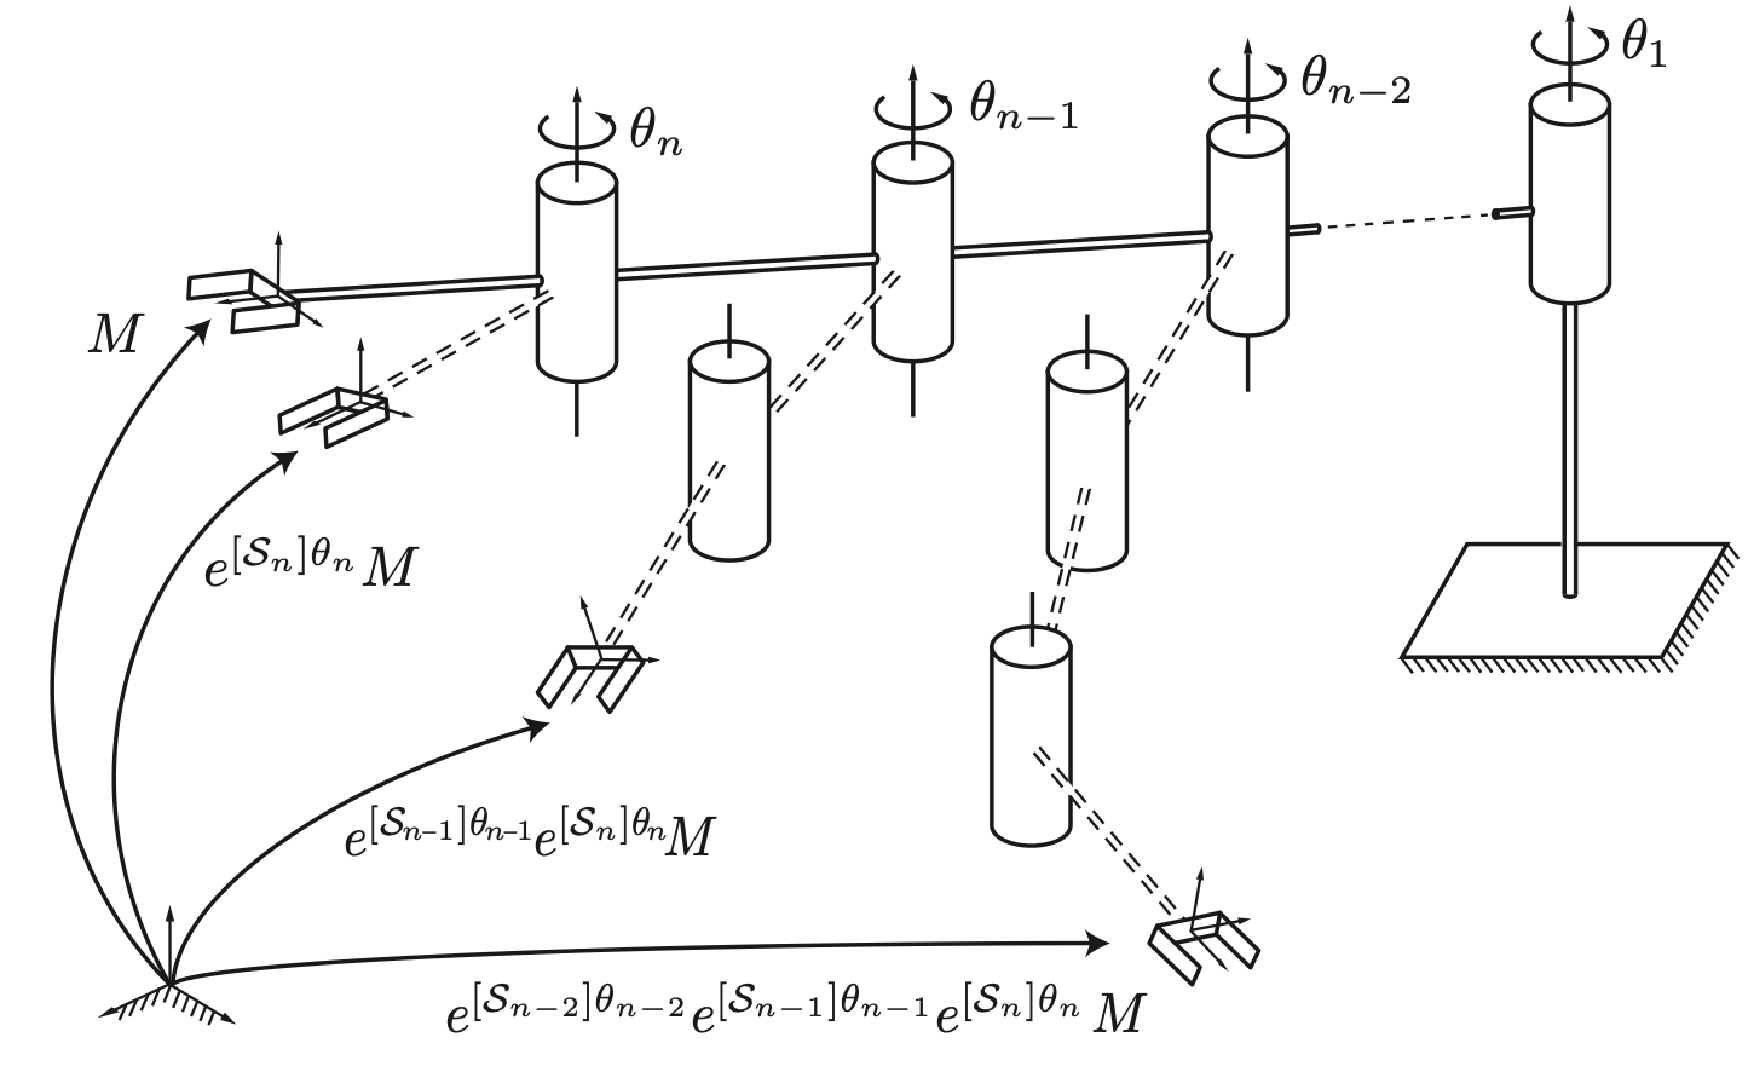
\includegraphics[width=0.7\textwidth]{assets/PoE_Visualization.pdf} 
  \caption{Visualization of PoE Formula}
  \label{fig:PoE_Visualization}
\end{figure}

\section{Task 4}

\subsection{Relation between DH-convention and PoE formula}
\subsection{DH-convention vs PoE formula - advantages and disadvanteges}
In this section we try to elaborate the differences between the DH convention and the PoE formula. Both methods differ in several points and have advantages and disadvantages. The DH convention on the one hand has fixed rules to attach frames to joints. This might sometimes seem to be exhaustig. Especially for complex robots with a lot of links it can become a tedious work. If all frames are attached properly one can easily find the homogenious transormations between all consecutive frames \(T_{1}^{0}\) to \(T_{n}^{n-1}\). Using the DH convention the homogenious transformations is established by using the minimal number of parameters to describe joint movements. The minimal number of parameters in the DH convention are  \(a_{i}, d_{i}, \alpha_{i}, \vartheta{i}\). These DH paramters can be used immediatlly to build the transformation matrix T. Multipling all these matrices returns the Transformation from base to end effector and the forward kinematics is solved. The easy establishment of the transformation matrix with the minimal number of parameters is the biggest advantage of the DH convention. Still there exist different DH conventions for attaching the frames to the links. This might sometimes be confusing. Another disadvatage is that the DH-parameters can become ill-conditioned. Especially in the special cases where consecutive joint axes are parallel or do intersect little changes in the robot geomety can make huge changes in the DH-parameters. Errors in manufacturing, CAD modells or in other areas can therefore lead to bigger problems. 

In contrast to that the PoE does not expect to attach frames at each joint. After deciding for a base and end effector frame and   establishing the M matrix, which defines the homegenious transformation from base to end effector in the robot's home position, one can use the PoE formula to solve the forward kinmetaics. There is a smaller effort when attaching frames to the robot and not a such a problem of ill-conditioned parameters. The interpretation of the joints as screw motion might be more intuitve. Besides that the PoE formula does not differ when using it for prismatic and rotational joints. In the DH convention the parameter \(d_{i}\) for prismatic joints and the parameter \(\vartheta{i}\) for rotational joints are variable. In these cases those DH-paramters are not solely determined by the geometry of the link. This is a disadvantage of the DH-convention. This problem does not appear in the PoE formula where prismatic and rotational joints are treated equally. Still, in the PoE-formula it might be more effort to establish the screw axis and applying the matrix exponential. When using a computer this disadvantage might be irrelevant. Besides that the PoE formula does not work with a minimal number of parameters. 



The PoE formula on the other hand does not expect frames to be attached to each link. 
\chapter{Here Comes Chapter 2}

\Blindtext

\begin{figure}
  \centering
  
\includegraphics[width=0.5\textwidth]{hovedlogo} 
  \caption{NTNU logo}
  \label{fig:logo2}
\end{figure}

\section{Title of section 2}








\chapter{Here Comes Chapter 3}

\Blindtext

\begin{figure}
  \centering
  
\includegraphics[width=0.5\textwidth]{hovedlogo} 
  \caption{NTNU logo}
  \label{fig:logo}
\end{figure}





\chapter{Conclusion}

\blindtext[4]



\printbibliography[title=References]

\appendix
\chapter{Name of Appendix} 

\section{This is a section}

\end{document}